\chapter{Implementation and Results}
\label{chap:Implementation}
\pagestyle{plain}
\vspace{0.5cm}

\noindent In this chapter is presented the overall description of the dataset used in the experiment and the related work already done.

\section{PMEmo dataset}
This thesis is based on the paper \textit{The PMEmo dataset for Music Emotion Recognition} \cite{zhang2018pmemo}. K. Zhang, H. Zhang and S.Li created a novel dataset called \gls{pmemo} containing emotions of 794 songs as well as \gls{eda} signals.
\\

Most researchers working on \gls{mer} adopt methods in supervised \gls{ml} to implement music emotion prediction \cite{yang2012machine}, which usually need a large number of songs with emotion labels provided by listeners to train the models.

A musical experiment was well-designed for collecting the affective annotated music corpus oh high quality, which recruited 457 subjects.
The dataset (about $1.3Gb$) is publicly available to the research community at \href{https://drive.google.com/drive/folders/1qDk6hZDGVlVXgckjLq9LvXLZ9EgK9gw0}{this link}\footnote{https://drive.google.com/drive/folders/1qDk6hZDGVlVXgckjLq9LvXLZ9EgK9gw0}.
\\
It is intended for benchmarking in \gls{mir} and \gls{mer}, it involves precomputed audio features sets and manually selected chorus excerpts (in .mp3) of songs, to facilitate the development of chorus-related research.

\subsection{Dataset structure}
The dataset contain $794$ music clips annotated by $457$ subjects, where participants come from different countries and majors, in order to eliminate the effects of cultural and educational background \cite{hu2017cross}.
\\
Chorus parts are manually selected from students majoring in music.
\\ \indent
Meanwhile, the \gls{eda} of subjects when listening to these music are also recorded, making it possible to analyze emotion states in multiple modes. All annotations are stored in CSV files delimited by comma.
\\
The dataset is composed of:
\begin{itemize}
	\item annotations: valence and arousal values for each song. There are:
	\begin{itemize}
		\item \textit{static\_annotations}: valence and arousal standard deviation values for each song, one value for each song.
		\item \textit{static\_annotations\_std}: valence and arousal mean values for each song, one value for each song.
		\item \textit{dynamic\_annotations}: valence and arousal standard deviation values for each song, acquired at a sampling rate of $2Hz$.
		\item \textit{dynamic\_annotations\_std}: valence and arousal mean values for each song, acquired at a sampling rate of $2Hz$.
	\end{itemize}
	\item chorus: all chorus excerpts of 794 songs manually selected.
	\item comments: songs comments taken from \href{https://music.163.com}{NetEase}\footnote{https://music.163.com} and \href{https://soundcloud.com}{SoundCloud}\footnote{https://soundcloud.com}.
	\item EDA: \gls{eda} data for each song, each one extracted by at least 10 subjects, with a sampling rate of $50Hz$.
	\item features: all features extracted by the authors of \cite{zhang2018pmemo}:
	\begin{itemize}
		\item \textit{EDA\_features}: features extracted from the EDA signals:
		\begin{itemize}
			\item \textit{EDA\_features\_static}: \gls{eda} static features for each song for each subject.
			\item \textit{EDA\_features\_dynamic}: \gls{eda} dynamic features for each song for each subject with a sampling rate of $50Hz$.
		\end{itemize}
		\begin{itemize}
			\item \textit{static\_features}: audio static features for each song.
			\item \textit{dynamic\_features}: audio dynamic features for each song with a sampling rate of $50Hz$.
		\end{itemize}
	\end{itemize}
	\item \textit{lrc\_dataset}: lyrics text of all music excerpts.
	\item lyrics:  lyrics text of all music excerpts divided by each timestamp.
	\item \textit{metadata}: metadata of the songs, containing \textit{music\_ID}, title, artist, album, duration, \textit{chorus\_start\_time} and \textit{chorus\_end\_time}.
\end{itemize}
\newpage
Since the early years of \gls{mer}, there have been numerous efforts to build datasets with emotional annotations, to facilitate the development and evaluation of music emotion recognition. Table \ref{table:datasets} from \cite{zhang2018pmemo} summarize some works on that.
\begin{savenotes}
\begin{table}[h!]
	\centering
	\begin{tabular}{|l|l|p{0.3\textwidth}|c|}
		\hline
		Name & Stimulus & Data & Audio\\ [0.5ex] 
		\hline\hline \href{http://www.projects.science.uu.nl/memotion/emotifydata/}{Emotify}\footnote{http://www.projects.science.uu.nl/memotion/emotifydata/}  & 400 excerpts & induced emotion & yes	\\ 
		\hline \href{http://music.ece.drexel.edu/research/emotion/moodswingsturk}{Moodswing}\footnote{http://music.ece.drexel.edu/research/emotion/moodswingsturk} & 240 excerpts (30s) & valence and arousal & no \\
		\hline \href{https://amg1608.blogspot.ca/}{Amg1608}\footnote{https://amg1608.blogspot.ca/} & 1608 excerpts (30s) & valence and arousal & no \\
		\hline \href{http://cvml.unige.ch/databases/emoMusic/}{emoMusic}\footnote{http://cvml.unige.ch/databases/emoMusic/} & 744 excerpts (45s) & valence and arousal & yes \\
		\hline \href{http://cvml.unige.ch/databases/DEAM/}{DEAM}\footnote{http://cvml.unige.ch/databases/DEAM/} & 1802 excerpts & valence and arousal & yes \\
		\hline \href{https://www.jyu.fi/hytk/fi/laitokset/mutku/en/research/projects2/pastprojects/coe/materials/emotion/soundtracks/Index}{SoundTracks}\footnote{https://www.jyu.fi/hytk/fi/laitokset/mutku/en/research/projects2/\newline pastprojects/coe/materials/emotion/soundtracks/Index} & 360 + 110 excerpts & valence, energy, tension, mood & yes \\
		\hline \href{https://hilab.di.ionio.gr/en/music-information-research/}{GMD}\footnote{https://hilab.di.ionio.gr/en/music-information-research/} & 1400 songs & genre, valence and arousal & yes \\
		\hline \href{http://www.eecs.qmul.ac.uk/mmv/datasets/deap/readme.html}{DEAPDataset}\footnote{http://www.eecs.qmul.ac.uk/mmv/datasets/deap/readme.html} & 120 music excerpts & valence, arousal, dominance and physiological data & no \\
		\hline PMEmo & 794 music chorus & valence, arousal and physiological data & yes \\
		\hline
	\end{tabular}
	\caption{Some existing music datasets with emotion annotations from \cite{zhang2018pmemo}}
	\label{table:datasets}
\end{table}
\end{savenotes}

\subsection{Song acquisition and subject selection}
They collected $1000$ songs from the "\textit{Billboard Hot 100}", the "\textit{iTunes top 100 songs}" and the "\textit{UK top 40 single charts}". They late discovered a set of duplicates and filtered double music obtaining a full song set of $794$ pop songs.
\\
Each datasets in \gls{mer} utilize music segments, here each clip is manually selected as one of the chorus parts of each song, which is implemented by university students in music major. The clips are of various length, exactly the duration of the chorus parts.
\\ \indent
A total of $457$ subjects, $236$ females and $221$ males were recruited to participate. Among them, $366$ are Chinese university students who are in non-music majors while $44$ are majoring in music recruited to ensure high quality labeling. To weaken the impact of cultural background, $47$ English speakers are invited to annotate the datasets.
\\
Each song received a total of at least $10$ emotion annotations including one by music-majoring and one by English speaker.

\subsection{Experiment design}
To monitor and obtain \gls{eda} continuously they used \href{https://www.biopac.com/product/eda-finger-transducer-bsl/}{MP150 Biopac system}\footnote{https://www.biopac.com/product/eda-finger-transducer-bsl/} with a sampling rate of $50Hz$ and export signals from \textit{AcqKnowledge} software.
\\
To annotate songs was developed a desktop application shown in figure \ref{fig:annotation_interface}. The annotation was done with the sliding area collecting dynamics annotations , from $1$ to $9$, at a sampling rate of $2Hz$. Annotators should make a statistic annotation for the whole music excerpts on nine-point scale after the dynamic labeling. Furthermore, annotators were asked to listen to the same music twice to annotate on valence and arousal separately.
\begin{figure}[h]
    \centering
    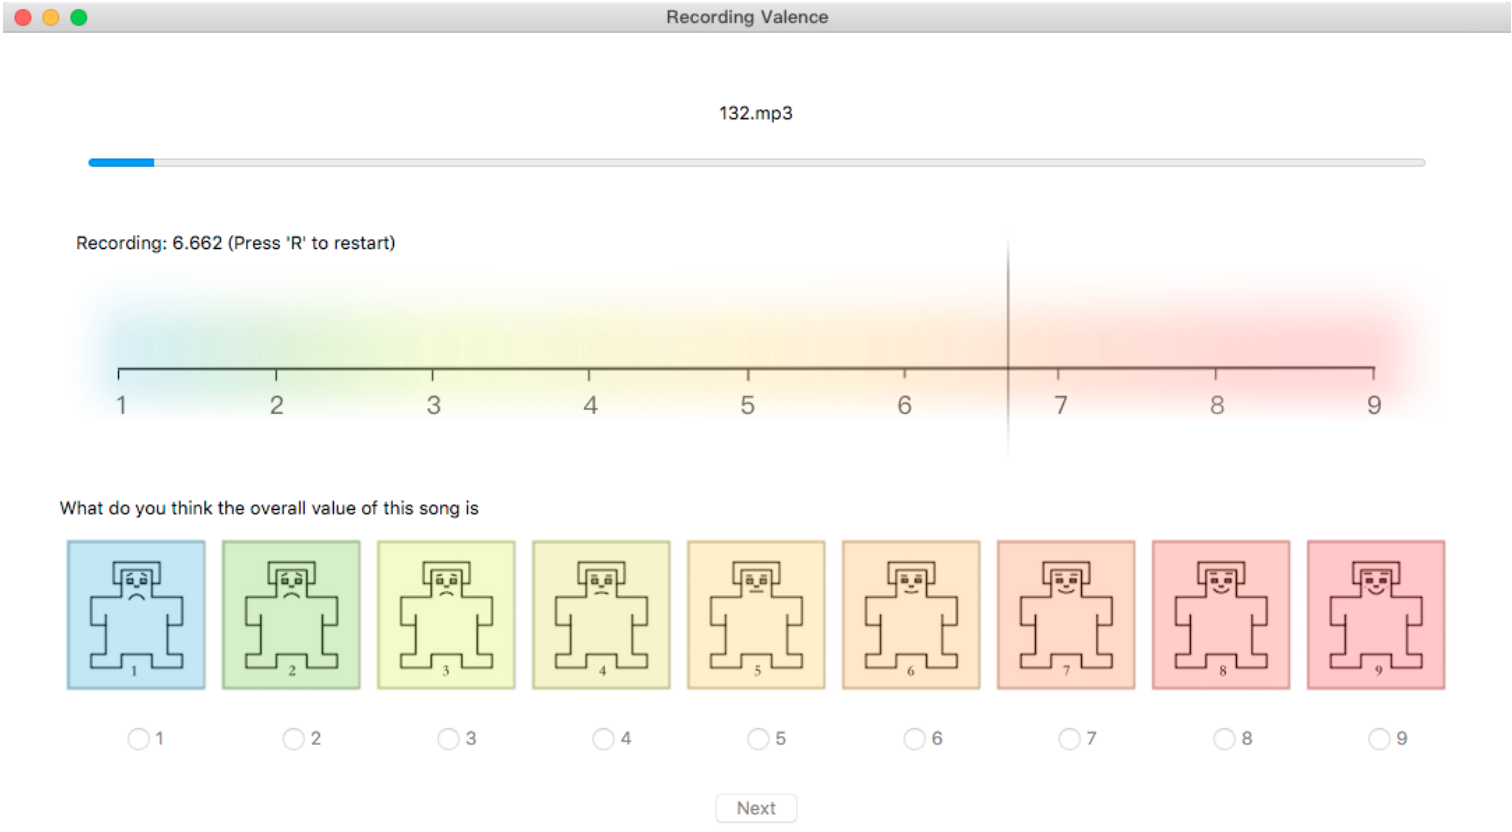
\includegraphics[width=0.65\textwidth]{annotation_interface.png} 
	\caption{Annotation interface for PMEmo}
    \label{fig:annotation_interface}
\end{figure}
\\
In figure \ref{fig:experimental_procedure} is shown the flow diagram of the experiment, where each subject spent $50$ minutes on average.
\begin{figure}[h]
    \centering
    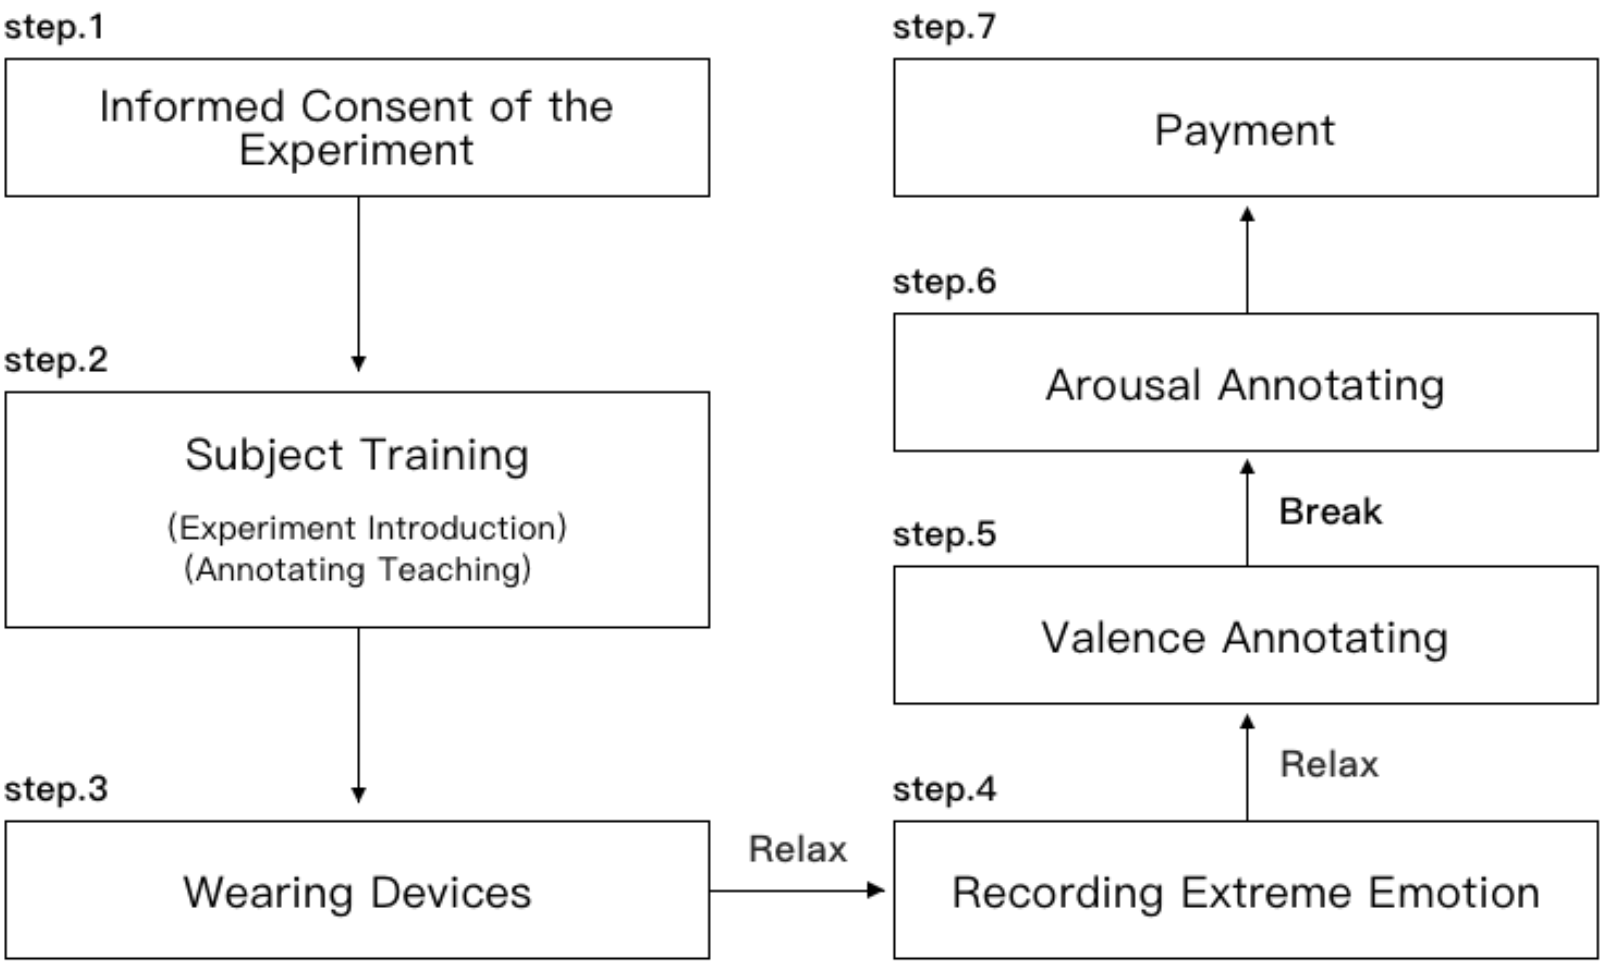
\includegraphics[width=0.7\textwidth]{experimental_procedure.png} 
	\caption{Experimental procedure for PMEmo}
    \label{fig:experimental_procedure}
\end{figure}
\\
Each subject listened to $20$ excerpts and one of those was duplicated to guarantee the high quality data as what was done in \cite{chen2015amg1608}. The annotations from this subjects were accepted only if the bias between duplicate clips were within $0.25$ in the \gls{va} space (they did not inform subjects about the duplicated excerpt).
\\
In total $457$ subjects have participated but $401$ were considered valid annotations ($87.7\%$). Each music clip was annotated by at least $10$ subjects including English speakers and semi-experts from music academy.

\subsection{Data reliability}
As \gls{iot} concept remarks, annotators need some preliminary time before they can give meaningful and reliable annotations. Schubert in \cite{schubert2013reliability} found that median \gls{iot} for valence was $8s$ while for arousal $12s$. Other researchers showed that annotations began to converge after $10s$. The \gls{pmemo} authors decided to discard first $15s$ for the dynamic annotations from the data.
\\ \indent
To evaluate annotation consistency they used the Chronbach's $\alpha$, it represent the degree to which a set of items measures a single unidimensional latent construct. In \cite{zhang2018pmemo} computed the Chronbach's $\alpha$ on the sequence of annotations for each song.
\\
They processed annotations by:
\begin{equation}
	a_{j,i}=a_{j,i}+(\bar{A}_j-\bar{A})
\end{equation}
where:
\begin{itemize}
	\item $a_{j,i}$ is the label annotated by subject $j$ at time $i$
	\item $\bar{A}$ is the mean of all the labels for this song by all subjects
	\item $\bar{A}_j$ is the mean of dynamic labels by subject $j$
\end{itemize}
The mean (averaged across songs) and the standard deviation of the Chronbach's $\alpha$ for the annotation in the \gls{pmemo} dataset are shown in table \ref{table:Chronbach}.
\begin{table}[h!]
	\centering
	\begin{tabular}{|c|c|c|}
		\hline
		Dimension & Mean value & Std Dev \\ [0.5ex] 
		\hline\hline Valence & 0.998 & 0.005 \\ 
		\hline Arousal & 0.998 & 0.008 \\ 
		\hline
	\end{tabular}
	\caption{Mean and standard deviation of the Chronbach's $\alpha$ for PMEmo dataset annotations}
	\label{table:Chronbach}
\end{table}

\subsection{Feature set}
As already mentioned before in \ref{music_features}, for generic \gls{mer} there has been no attempt made at defining a "standard" feature set. In PMEmo work \cite{zhang2018pmemo} they based on the INTERSPEECH 2013 \gls{compare} \cite{schuller2013interspeech} and extracted a feature set of 6373-dimension scale.
\\
They provided all $6373$-dimension features in song level for the sake of static emotion task. They extracted only the core of $260$-dimension features in segment level (calculated in $1s$ window with $0.5s$ overlap) for dynamic recognition task to properly reduce the computing load.
\\
Extraction of the features is done with the open-source toolkit \href{https://www.audeering.com/opensmile/}{openSMILE}\footnote{https://www.audeering.com/opensmile/} \cite{eyben2013recent}.
\\
No feature selection procedure was implemented in \gls{pmemo} work.

\subsection{PMEmo performances}
In the article, they adopt \gls{mlr} and \gls{svr} as the base classifiers to model emotions in valence and arousal.
\\
For the static part, they trained and tested the classifiers using all the $6373$-dimension features $x_1,x_2,...,x_{6373}$ and separate static labels of valence $y_{valence}$ and arousal $y_{arousal}$ respectively.
\begin{equation}
	{X_1,X_2,...,X_m} \quad \rightarrow \quad {e_1,e_2,...,e_m}
\end{equation}
where:
\begin{itemize}
	\item $m$ is the number of songs
	\item $X_i={x_1,x_2,...,x_{6373}}$ is the feature set of the $i^{th}$ song
	\item $e_i$ is the value of valence or arousal for this song
\end{itemize}
With respect of continuous mood of a song, is natural to consider a decoupling into two scales and then recognize them separately.
\\
For the dynamic emotion, defined as:
\begin{equation}
	L_i=\bar{L}_i+D_i^{t_i}
\end{equation}
where:
\begin{itemize}
	\item $t_i$ is the number of timestamps in the $i^{th}$ song
	\item $\bar{L}_i$ is the mean of dynamic emotion
	\item $D_i^{t_i}$ is the fluctuation at each timestamp
\end{itemize}
the global model is:
\begin{equation}
	{X_1,X_2,...,X_m} \quad \rightarrow \quad {\bar{L}_1,\bar{L}_2,...,\bar{L}_m}
\end{equation}
while, the local model is:
\begin{equation}
	{Y_1^{t_1},Y_2^{t_2},...,Y_m^{t_m}} \quad \rightarrow \quad {D_1^{t_1},D_2^{t_2},...,D_m^{t_m}}
\end{equation}
where:
\begin{itemize}
	\item $m$ is the number of songs
	\item $X_i$ is the global feature set of it
	\item $Y_i^{t_i}$ is a matrix of 260 columns and $t_i$ rows
\end{itemize}
Before the regression models, they resized all the annotations (both for static and dynamic annotations) into $[0,1]$.
\\ \indent
Static task is to predict the overall emotion of a whole song, represented by a single valence value and arousal value. To train and test, they divided the dataset in $11$ folds, 10 constituted the training set and the remaining set used to test the train model. A 10-fold-cross-validation was used for parameter optimization.
\\
\gls{rmse} and Pearson Correlation Coefficient (r) were calculated separately for valence and arousal. In table \ref{table:PMEmo_results_static} is shown results on static emotions.
\begin{table}[h!]
	\centering
	\begin{tabular}{|c|c|c|c|}
		\hline
		Dimension & Classifier & RMSE & r \\ [0.5ex] 
		\hline\hline Valence & MLR & 0.136 & 0.546 \\ 
		\hline Valence & SVR & 0.124 & 0.638 \\
		\hline Arousal & MLR & 0.111 & 0.719 \\
		\hline Arousal & SVR & 0.102 & 0.764 \\
		\hline
	\end{tabular}
	\caption{Evaluation results on static emotions}
	\label{table:PMEmo_results_static}
\end{table}
\\
About the dynamic case, a hierarchical regression model aiming to recognize the global trend as well as local variation was built. For Global-scale they extracted, for each song, one global feature and mapped it into one global emotion. For Local-scale operation, for each song, they divided it into $1s$ segment with $50\%$ overlap, then extracting the local features from these fragments and project them onto mood space.
\\
In table \ref{table:PMEmo_results_dynamic} is presented the evaluation results on dynamic emotions.
\begin{table}[h!]
	\centering
	\begin{tabular}{|c|c|c|c|c|}
		\hline
		Dimension & Classifier & Scale & RMSE & r \\ [0.5ex] 
		\hline\hline Valence & MLR & global & 0.103 & 0.673 \\
		\hline Valence & MLR & local & 0.016 & 0.047 \\
		\hline Valence & SVR & global & 0.106 & 0.675 \\
		\hline Valence & SVR & local & 0.016 & 0.095 \\
		\hline Arousal & MLR & global & 0.113 & 0.816 \\
		\hline Arousal & MLR & local & 0.020 & 0.103 \\
		\hline Arousal & SVR & global & 0.101 & 0.844 \\
		\hline Arousal & SVR & local & 0.019 & 0.115 \\
		\hline
	\end{tabular}
	\caption{Evaluation results on dynamic emotions}
	\label{table:PMEmo_results_dynamic}
\end{table}
\\
In \gls{pmemo} work, as already mentioned, they also recorded \gls{eda} subjects data when they were listening to music.
\\
On \gls{eda}, they employed a low-pass filter of $0.6Hz$ to diminish the noise due to motion artifacts. Then skin electric conductance was scaled in z-score:
\begin{equation}
	z-score=\dfrac{X-\mu}{\sigma}
\end{equation}
where $\mu$ is the mean of vector $X$ and $\sigma$ is the standard variation.
Last passage on \gls{eda} signal was to resample them, from $50Hz$ to $2Hz$ due to different acquisition of EDA and continuous emotions.
\\
They trained and tested \gls{mlr} and \gls{svr} with pre-processed \gls{eda} data in the dynamic case and results are shown in table \ref{table:PMEmo_results_EDA}.
\begin{table}[h!]
	\centering
	\begin{tabular}{|c|c|c|c|c|}
		\hline
		Dimension & Classifier & Scale & RMSE & r \\ [0.5ex] 
		\hline\hline Valence & MLR & global & 0.139 & 0.063 \\
		\hline Valence & MLR & local & 0.016 & 0.060 \\
		\hline Valence & SVR & global & 0.141 & 0.017 \\
		\hline Valence & SVR & local & 0.016 & 0.059 \\
		\hline Arousal & MLR & global & 0.186 & 0.011 \\
		\hline Arousal & MLR & local & 0.019 & 0.097 \\
		\hline Arousal & SVR & global & 0.194 & 0.040 \\
		\hline Arousal & SVR & local & 0.019 & 0.099 \\
		\hline
	\end{tabular}
	\caption{Evaluation results on dynamic EDA}
	\label{table:PMEmo_results_EDA}
\end{table}





